\documentclass[a4paper,11pt]{article}
\usepackage[T1]{fontenc}
\usepackage[utf8]{inputenc}
\usepackage{lmodern}
\usepackage{graphicx}
\usepackage{float}

\title{Sudoku}
\author{Dominik Danter}

\begin{document}

\maketitle
\tableofcontents

\begin{abstract}
\end{abstract}

\section{Introduction}
Sudoku is a logic-based, combinatorial number-placement puzzle. The objective is to fill a 9x9 grid with digits so that each column, each row, and each of the nine 3x3 sub-grids that compose the grid (also called "boxes", "blocks", "regions", or "sub-squares") contains all of the digits from 1 to 9. The puzzle setter provides a partially completed grid, which typically has a unique solution.

Completed puzzles are always a type of Latin square with an additional constraint on the contents of individual regions. For example, the same single integer may not appear twice in the same 9x9 playing board row or column or in any of the nine 3x3 subregions of the 9x9 playing board.

The puzzle was popularized in 1986 by the Japanese puzzle company Nikoli, under the name Sudoku, meaning single number. It became an international hit in 2005.
\cite{wikipedia}

\section{Gameplay}

\subsection{Main Window} 


On the top left you'll see two menus:

\begin{itemize}
  \item File
  \item Cheat
\end{itemize}

At the center of the sreen is the board. You can enter a number between 1 and 9 into a field that was empty at the beginnig of the game by clicking into the cell and pressing a number on your keyboard. 

At the bottom you have 

\begin{itemize}
  \item the \textit{new} game button.
  \item the \textit{reset} game button.
  \item the counter.
  \item the \textit{show doubles} option. 
\end{itemize}


\begin{figure}[H]
  \begin{center}
    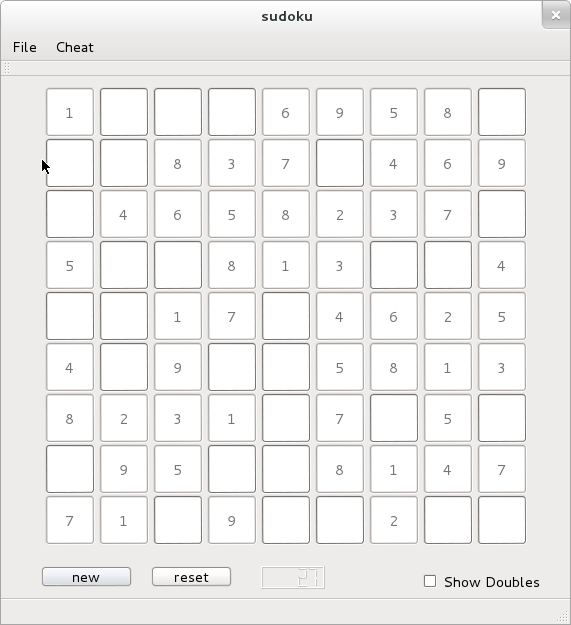
\includegraphics{img/mainWindow.png}
    \label{fig:}
    \caption{the main window}
  \end{center}
\end{figure}

\subsection{New game}
When you start the programm you will be presented with the 9x9 playing board. It will have already been initialised with an easy setup. If you wish to play at a different level you can do so any time by pressing the "new game" button. A new window will pop up. There you can choose between three levels. Easy, ``Medium'' and ``Hard''. Please do note, that a medium and especially a hard board may take some time to be generated. 

\subsection{Resetting the game}

You can always reset the board to it's initial state by simply pressing the ``reset'' button located on the left bottom of the main window. This is \textbf{not} a form of cheating.

\subsection{Loading and saving}

A board can be saved at any stage of the game. The menu items can be accessed through the ``File'' menu located at the top left corner. 
Naturally you can also load a game that you have previously saved. A loaded game however can never be eligible for making it into the highscore.


\subsection{Cheating}
By means of the cheating menu located on the top left corner, you can choose to receive some additional help. But be aware once you have received such help you will no longer be eligible to get yourself into the highscore. There are currently two forms of help available

\begin{itemize}
  \item Get Field
  \item Solve
\end{itemize}

The option ``Get field'' will randomly choose a field that is without value and fill it out for you, whereas ``Solve'' will solve the whole board for you.

Please be aware that loading a game, is also a way of cheating (as described above).

\subsection{Show Doubles}

If you check the ``show doubles'' check box a visiual aid will be provided. All cells that are in an invalid state will be marked. This is \textbf{not} a form of cheating.

\begin{figure}[H]
  \begin{center}
    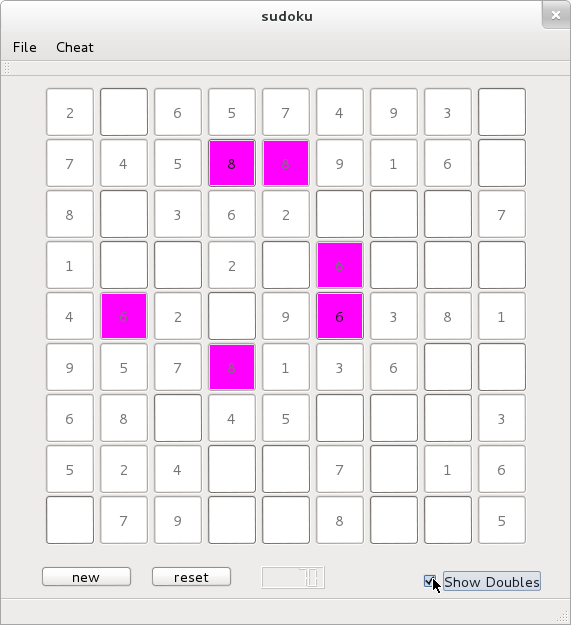
\includegraphics{img/showDoubles.png}
    \label{fig:}
    \caption{All invalid fields are marked.}
  \end{center}
\end{figure}

\subsection{Highscore}

If you complete your board fast enough, you make it into the Highscore. The 10 fastest player will be eligible, a higher level of difficulty always outweighs a faster time. This means if there have been 10 or more succesful attempts on completing a board at the level medium without cheating, there is no way that even a lightning fast completion of an easy board can make it into the highscore. There is however always a chance for a game that is played at level hard to achieve such honor.

\begin{figure}[H]
  \begin{center}
    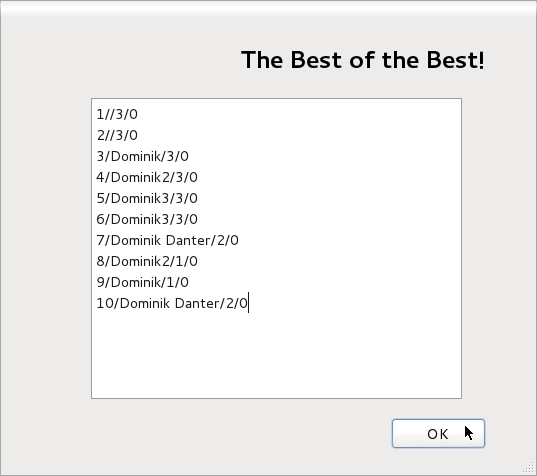
\includegraphics{img/highScore.png}
    \label{fig:}
    \caption{Congrats, you have made it!}
  \end{center}
\end{figure}

You know that you have made it, if the game prompts you for your name.
\begin{figure}[H]
  \begin{center}
    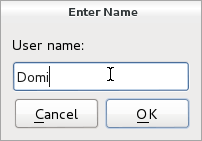
\includegraphics{img/enterName.png}
    \label{fig:}
    \caption{Just enter your name.}
  \end{center}
\end{figure}


\end{document}
